\documentclass[11pt,a4paper]{article}
\usepackage{fontspec}
\setmainfont{Source Serif 4}[Path=/home/claude/ref/fonts/, UprightFont=SourceSerif4-Regular.ttf, BoldFont=SourceSerif4-Semibold.ttf, ItalicFont=SourceSerif4-It.ttf]
\setmonofont{IBM Plex Mono}[Path=/home/claude/ref/fonts/, UprightFont=IBMPlexMono-Regular.ttf, BoldFont=IBMPlexMono-Medium.ttf, Scale=0.88]
\usepackage[a4paper,margin=2.4cm]{geometry}
\usepackage{amsmath}
\usepackage{graphicx,booktabs,float,caption,array,xcolor,longtable}
\usepackage{xurl}
\usepackage[hidelinks]{hyperref}
\usepackage[round]{natbib}
\usepackage{setspace}
\setstretch{1.08}
\renewcommand{\topfraction}{0.9}
\renewcommand{\bottomfraction}{0.8}
\renewcommand{\textfraction}{0.1}
\renewcommand{\floatpagefraction}{0.75}
\setlength{\parindent}{0pt}
\setlength{\parskip}{0.55em}
\captionsetup{font=small,labelfont=bf}
\setlength{\bibsep}{3pt}
\urlstyle{same}
\hypersetup{pdftitle={Lost Kingdoms on the High Street},pdfauthor={Dr Tristan Hotham}}

\begin{document}
\begin{center}
{\Large\bfseries Lost Kingdoms on the High Street: Early Medieval Kingdom Names in Modern British Business Names\par}
\vspace{1.2em}
{\large Dr Tristan Hotham\par}
\vspace{0.3em}
{\small Independent researcher\\
ORCID: 0000-0003-4931-9349\\
DOI: https://doi.org/10.5281/zenodo.24104340\par}
\vspace{0.8em}
2026
\end{center}

\begin{quote}
\small
\begin{center}\textbf{Abstract}\end{center}
The kingdoms of early medieval Britain disappeared more than a thousand years ago, but their names are on shop fronts, pubs, police stations and street signs. Do these names still sit where the kingdoms were? I read every UK feature in OpenStreetMap named after one of twelve early medieval kingdoms, from Wessex and Mercia to Elmet and Rheged, classified 1,087 named features as businesses and voluntary bodies, public bodies, streets or other objects, and compared their locations with approximate extents of the kingdoms around AD 800, drawn as unions of modern areas and fixed, with the analysis plan, before any feature was located. Against a baseline of census residents, kingdom names on businesses, clubs and societies are concentrated inside their kingdoms: 75 of 95 Wessex names lie inside an extent holding 10.0\% of UK residents (rate ratio per resident 34, 95\% CI 20 to 71), 30 of 32 Mercia names lie inside Mercia and all 33 Northumbria names inside Northumbria. Pooled across the three names with enough cases, the rate ratio is 44 (CI 19 to 100), and it stays above 14 in all 19 planned robustness checks; a placebo with the wrong kingdoms' extents shows no concentration (0.97, CI 0.51 to 1.83). Public bodies are not detectably more local than businesses, but streets travel further: only 52\% of kingdom-named streets are inside the kingdom. Most names that leave travel only a few kilometres. The data are observational, cover only mapped features and cannot date the names.

\textbf{Keywords:} place names; commercial names; regional identity; early medieval kingdoms; Anglo-Saxon England; OpenStreetMap; toponymy
\end{quote}

\section{Introduction}
Early medieval Britain was a patchwork of kingdoms. Some, such as Wessex, Mercia and Northumbria, grew large and are familiar from school history; others, such as Elmet around Leeds, Rheged near the Solway, Lindsey in north Lincolnshire, Strathclyde on the Clyde and Dál Riata across Argyll and Antrim, were smaller, shorter lived or absorbed by their neighbours \citep{yorke1990,bassett1989,rollason2003,clarkson2014}. None of them survives as a unit of government. Yet their names are everywhere. There is a West Mercia Police and a Northumbria Police, a Wessex Water and a Northumbrian Water, a Mercian Regiment and a Northumbria University, and below them a long tail of private names: the Wessex Kia dealer, the Earl of Mercia pub, Northumbrian Heritage Meats, Elmet Fisheries, the Rheged centre near Penrith.

This paper asks a simple geographical question about that tail. When a business, club or society takes a kingdom's name, does it do so inside the kingdom? Or have the names, once revived, become free-floating brands that anyone anywhere can use? The answer matters for two literatures. For the study of regional identity, the persistence of an early medieval name inside its old territory would be evidence that the name still works as a regional label, that people choose it because it says where they are \citep{paasi1986,paasi2003}. For the study of commercial and street naming, which has shown how names are chosen for their meaning, their commemorative weight and their market value \citep{roseredwood2010,lightyoung2015}, kingdom names are an unusually clean case: they have a known, if fuzzy, home territory, they are not the names of any current administrative unit, and their uptake is voluntary.

There are good reasons to expect the names to have travelled. One revival, Thomas Hardy's, was literary: Hardy wrote that he had ``ventured to adopt the word `Wessex' from the pages of early English history'' for his fiction and that the press and public had taken it up \citep{hardy1895,gatrell2003}. A literary or romantic name can attach to anything, anywhere. Businesses move, chains expand and founders carry names with them. On the other hand, a name like Mercia or Northumbria means little to customers who do not feel they live in it, so firms that want a regional label have reason to use the local one.

I measure where kingdom names are used by reading every matching feature in OpenStreetMap, the open, volunteer-built map of the world \citep{haklay2008}. From 7,500 UK features whose names contain county, rose or kingdom words, retrieved through the QLever SPARQL engine \citep{bast2017,bast2021}, I keep the 1,087 that contain one of twelve kingdom names as a whole word, read each one, and classify it as a business or voluntary body (shops, pubs, firms, clubs, societies, charities and places of worship), a public body (police, councils, schools, universities, the armed forces, statutory utilities), a street, a named building or site, or something else (bus stops, railway lines, substations, signs). I then compare the locations of these features with approximate extents of the kingdoms around AD 800, drawn as unions of modern areas following the standard historical maps \citep{hill1981,yorke1990}, in three versions (heartland, main, widest). The extents, the classification rules, the outcome, the baseline and the tests were written down in an analysis plan before any feature was located against any extent.

The main result is clear. Kingdom names on businesses and voluntary bodies are heavily concentrated inside their kingdoms. Pooled across the three names with at least 20 such features (Wessex, Mercia and Northumbria), there are 44 times as many per resident inside the main extent as outside. Every planned robustness check gives a rate ratio of at least 14.5, and a placebo that measures each name against the wrong kingdom finds nothing. The names that leave mostly do not go far: of the 20 Wessex names outside the main extent, 14 are within 25 km of its edge, most of them in Bristol and in Cardiff and Newport, across rivers that the extent treats as borders. Public bodies are not detectably more local than private names, but streets, which councils and developers name, are much less local.

The contribution is threefold. First, it offers a systematic, map-wide measurement of where early medieval kingdom names are used today, with every case read and published. Second, it offers a transparent design for this kind of question, a rate ratio per resident inside an approximate historical extent, with uncertainty from resampling brands rather than branches, that can be applied to other historical regions. Third, it separates kinds of naming decision: a business choosing its own name behaves differently from a developer naming a street. The study is descriptive and correlational, and it cannot say why the names stay at home.

Section~\ref{sec:lit} reviews work on the kingdoms, on regional identity and on commercial and street naming. Section~\ref{sec:data} describes the data and the curation, Section~\ref{sec:design} the pre-specified design, Section~\ref{sec:results} the results and Section~\ref{sec:robust} the checks. Section~\ref{sec:disc} discusses interpretation and limitations, and Section~\ref{sec:conc} concludes.

\section{Background and literature}\label{sec:lit}
\subsection{The kingdoms and their extents}
The political map of Britain between the end of Roman rule and the Viking age is reconstructed from a thin documentary record, archaeology and later administrative geography. The standard synthesis for the English kingdoms is \citet{yorke1990}, with the essays in \citet{bassett1989} on how kingdoms formed and the maps in \citet{hill1981}, which remain a standard cartographic reference. These works agree on the broad picture used here: several English kingdoms of very different sizes, with British kingdoms to the west and north, and boundaries that moved through conquest, marriage and overlordship.

Wessex grew from the upper Thames and Hampshire to cover the south west, and from the ninth century came to dominate southern England \citep{yorke1990}. Mercia, centred on the upper Trent, became the dominant Midland kingdom and at its height drew Lindsey, the Hwicce and other peoples into its orbit \citep{brownfarr2001}. Northumbria was formed from two kingdoms, Deira between the Humber and the Tees and Bernicia to the north, and at its greatest extent stretched from the Humber to the Forth \citep{rollason2003}. Lindsey, the northern part of later Lincolnshire, had its own kings before it was absorbed \citep{vince1993}. East Anglia, the kingdom of the East Angles in Norfolk and Suffolk, is unusual among these names because ``East Anglia'' is also in everyday use for a modern region.

The British kingdoms are harder to place. Elmet, around Leeds, was absorbed by Northumbria in the early seventh century \citep{yorke1990}; its name survives in places such as Sherburn in Elmet and Barwick in Elmet, and in modern culture, notably in the poems and photographs of \citet{hughes1979}. Rheged is placed near the Solway, though its extent is uncertain \citep{mccarthy2002}. Strathclyde, the kingdom of the Clyde, outlived the others and later expanded southwards \citep{clarkson2014}. Dál Riata spanned Argyll and the north of County Antrim; \citet{campbell2001} argues that the traditional story of Irish migration into Argyll is better read as an elite origin myth than as the record of a population movement. Dumnonia covered Devon and Cornwall \citep{pearce1978,pearce2004}.

Two points matter for what follows. The extents are approximate and contested, so any measurement must be robust to how they are drawn; and several overlap in time and space (Deira and Bernicia within Northumbria; Elmet and Rheged within Northumbria's later extent; Lindsey within Mercia's; Dumnonia within Wessex's later extent). The design therefore uses three versions of each extent and measures each name only against its own kingdom.

\subsection{Regions, identity and revived names}
In \citeauthor{paasi1986}'s account of how regions are institutionalised, a region acquires a territorial shape, a symbolic shape (a name and symbols), an institutional shape and finally a place in collective consciousness \citep{paasi1986}; regional identity is something made and remade rather than a fixed inheritance \citep{paasi2003}. Revived kingdom names fit this account closely. They are symbolic shapes without a current territory, attached in the modern period to institutions (police forces, water companies, regiments, universities) and to commercial life. Whether the names are anchored to their old territories, or have been detached from them, is an empirical question that this framework raises but does not answer. Work on regional identification in British politics finds that where people feel they belong shapes how they respond to local candidates \citep{collignonsajuria2018}, which suggests that regional labels carry meaning for ordinary people, not only for institutions.

\subsection{Commercial and street naming}
Critical place-name studies have moved from the etymology of names to the politics and economics of naming \citep{roseredwood2010}. Street names have been used to study commemoration and political change \citep{azaryahu1996,alderman2000,light2004,lightyoung2014} and, at scale, as data on culture and values \citep{otoperalias2018,bancilhon2021,gutierrez2022}. \citet{lightyoung2015} argue that place names now carry economic value, with corporate and commercial interests shaping urban naming. Business names are the most commercial of names: the owner chooses them, usually to signal something to customers. A regional or historical name can signal locality, heritage or quality, or simply sound good. Business names have been used much less than street names as geographical data, partly because complete, georeferenced registers of business names are hard to obtain. OpenStreetMap offers an imperfect but open alternative.

\subsection{OpenStreetMap as a source}
OpenStreetMap is built by volunteers. Its positional accuracy for roads in England compares well with the Ordnance Survey, but its completeness is uneven, better in cities and in more affluent areas \citep{haklay2010}. For points of interest such as shops and pubs the coverage is less studied and certainly incomplete. For this study the key question is whether coverage differs between the inside and the outside of the kingdoms in a way that could create the pattern. Section~\ref{sec:robust} addresses this with checks that change the baseline from residents to land area, leave out each region in turn, and use a placebo with other kingdoms' extents, which shares any coverage pattern but not the hypothesised link.

\section{Data}\label{sec:data}
\subsection{Named features}
The source is a QLever query of the OpenStreetMap planet \citep{bast2017,bast2021} for UK features whose name contains any of a list of county, rose and kingdom words, retrieved in 2026, with the name, the tags \texttt{shop}, \texttt{amenity}, \texttt{office}, \texttt{craft}, \texttt{leisure} and \texttt{highway}, and the geometry. The file has 7,500 rows (Section~\ref{sec:disc} discusses whether it is complete). I matched each kingdom name as a whole word, with its adjective where one is in use (Mercian, Northumbrian, East Anglian, Elmete, Deiran, Bernician, Dalriadan): whole-word matching removes the many raw hits for ``Commercial'' (which contains ``mercia'') and ``Madeira'' (``deira''). This leaves 2,547 matched OpenStreetMap objects. Each object was given a representative point inside its geometry.

\subsection{Classification and reading by eye}
Every object that is not a street was read by eye, and the decisions are in \texttt{code/overrides.csv}. The rules, in order, were: features tagged as highways are streets, except stops and paths; transport routes, railway lines, substations and other infrastructure, signs, memorials and artworks are ``other''; names built on a street name (``Wessex Road Surgery'', ``Northumbria Way Pharmacy'') are ``other'', because the kingdom name came from the street; tagged shops, crafts and tagged amenities, offices and leisure venues are businesses and voluntary bodies (``private'' for short) unless they are public bodies; public bodies are police and probation, fire and ambulance, councils, NHS and other health bodies, schools, colleges and universities, the armed forces, statutory water companies and drainage boards, and protected landscapes; untagged features with company, club, hotel or society words are private; untagged building names, estates and business parks are a separate ``site'' class. Duplicates (a pub mapped as a point and as a building) were merged when the same normalised name occurred within 250 m (1 km for street segments). Chains were given a common brand key, so that, for example, the 56 East Anglia shops include many branches of one children's hospice charity.

Three kinds of hand decision affect what counts as a kingdom name. Some matches are not the kingdom at all: ``Deira'' in a restaurant name is a district of Dubai, and ``Lindsey'' is also a first name and the name of a village in Suffolk and of Norton Lindsey in Warwickshire, so personal-name uses and anything within 3 km of those two villages were excluded (a rule fixed before the extents were used). Some names are place-derived: they come from a modern place that itself takes its name from the kingdom (Sherburn in Elmet, Barwick in Elmet, Kirton in Lindsey, the East and West Lindsey districts, Strathclyde Park); these are kept, flagged and dropped in a check. Ten Lindsey names that could be personal names were flagged as ambiguous and are also dropped in that check. In all, 136 matched objects (5.3\%) were changed or flagged by hand. Table~\ref{tab:flow} shows the flow from raw rows to the analysis sample.

\begin{table}[tbp]\centering\small\caption{From raw rows to the analysis sample.}\label{tab:flow}\begin{tabular}{lr}\toprule Step & Number\\\midrule
OpenStreetMap rows with a county, rose or kingdom word in the name & 7,500\\
Objects matching a kingdom name as a whole word & 2,547\\
Named features after merging duplicates (twelve names) & 1,087\\
\quad businesses and voluntary bodies (private) & 254\\
\quad public bodies & 93\\
\quad streets & 336\\
\quad named buildings and sites & 62\\
\quad other (stops, routes, infrastructure, signs; not the kingdom) & 342\\\midrule
Private features, eleven kingdom names (East Anglia apart) & 198\\
\quad distinct brands & 165\\
\quad place-derived (kept; dropped in R5) & 14\\
Objects changed or flagged by hand & 136 (5.3\%)\\
Areal units (MSOA, Scottish councils, NI districts) & 7,307\\\bottomrule\end{tabular}\end{table}

\subsection{Kingdom extents}
There are no agreed boundaries for these kingdoms, and the analysis does not pretend otherwise. I drew each kingdom as a union of modern areal units following the standard maps \citep{hill1981,yorke1990} and the specialist works cited above, in three versions: a heartland (core), the main extent around AD 800, and a widest plausible extent before about 900 (Appendix Table~\ref{tab:ext}). The units are MSOAs of 2021 in England and Wales (7,264 small areas, assigned to their ceremonial county or their 2021 district), council areas in Scotland and council districts in Northern Ireland, 7,307 units in all. Using modern units makes the extents reproducible and lets the baseline be counted exactly; it also means each extent follows modern county lines rather than the rivers and watersheds that probably mattered. For example, the main Wessex extent includes Somerset (with Bath and North Somerset) but not Bristol, which lies mostly north of the Avon and is assigned to Mercia; the wide extent adds Bristol. Figure~\ref{fig:map} shows the main extents.

\begin{figure}[tbp]\centering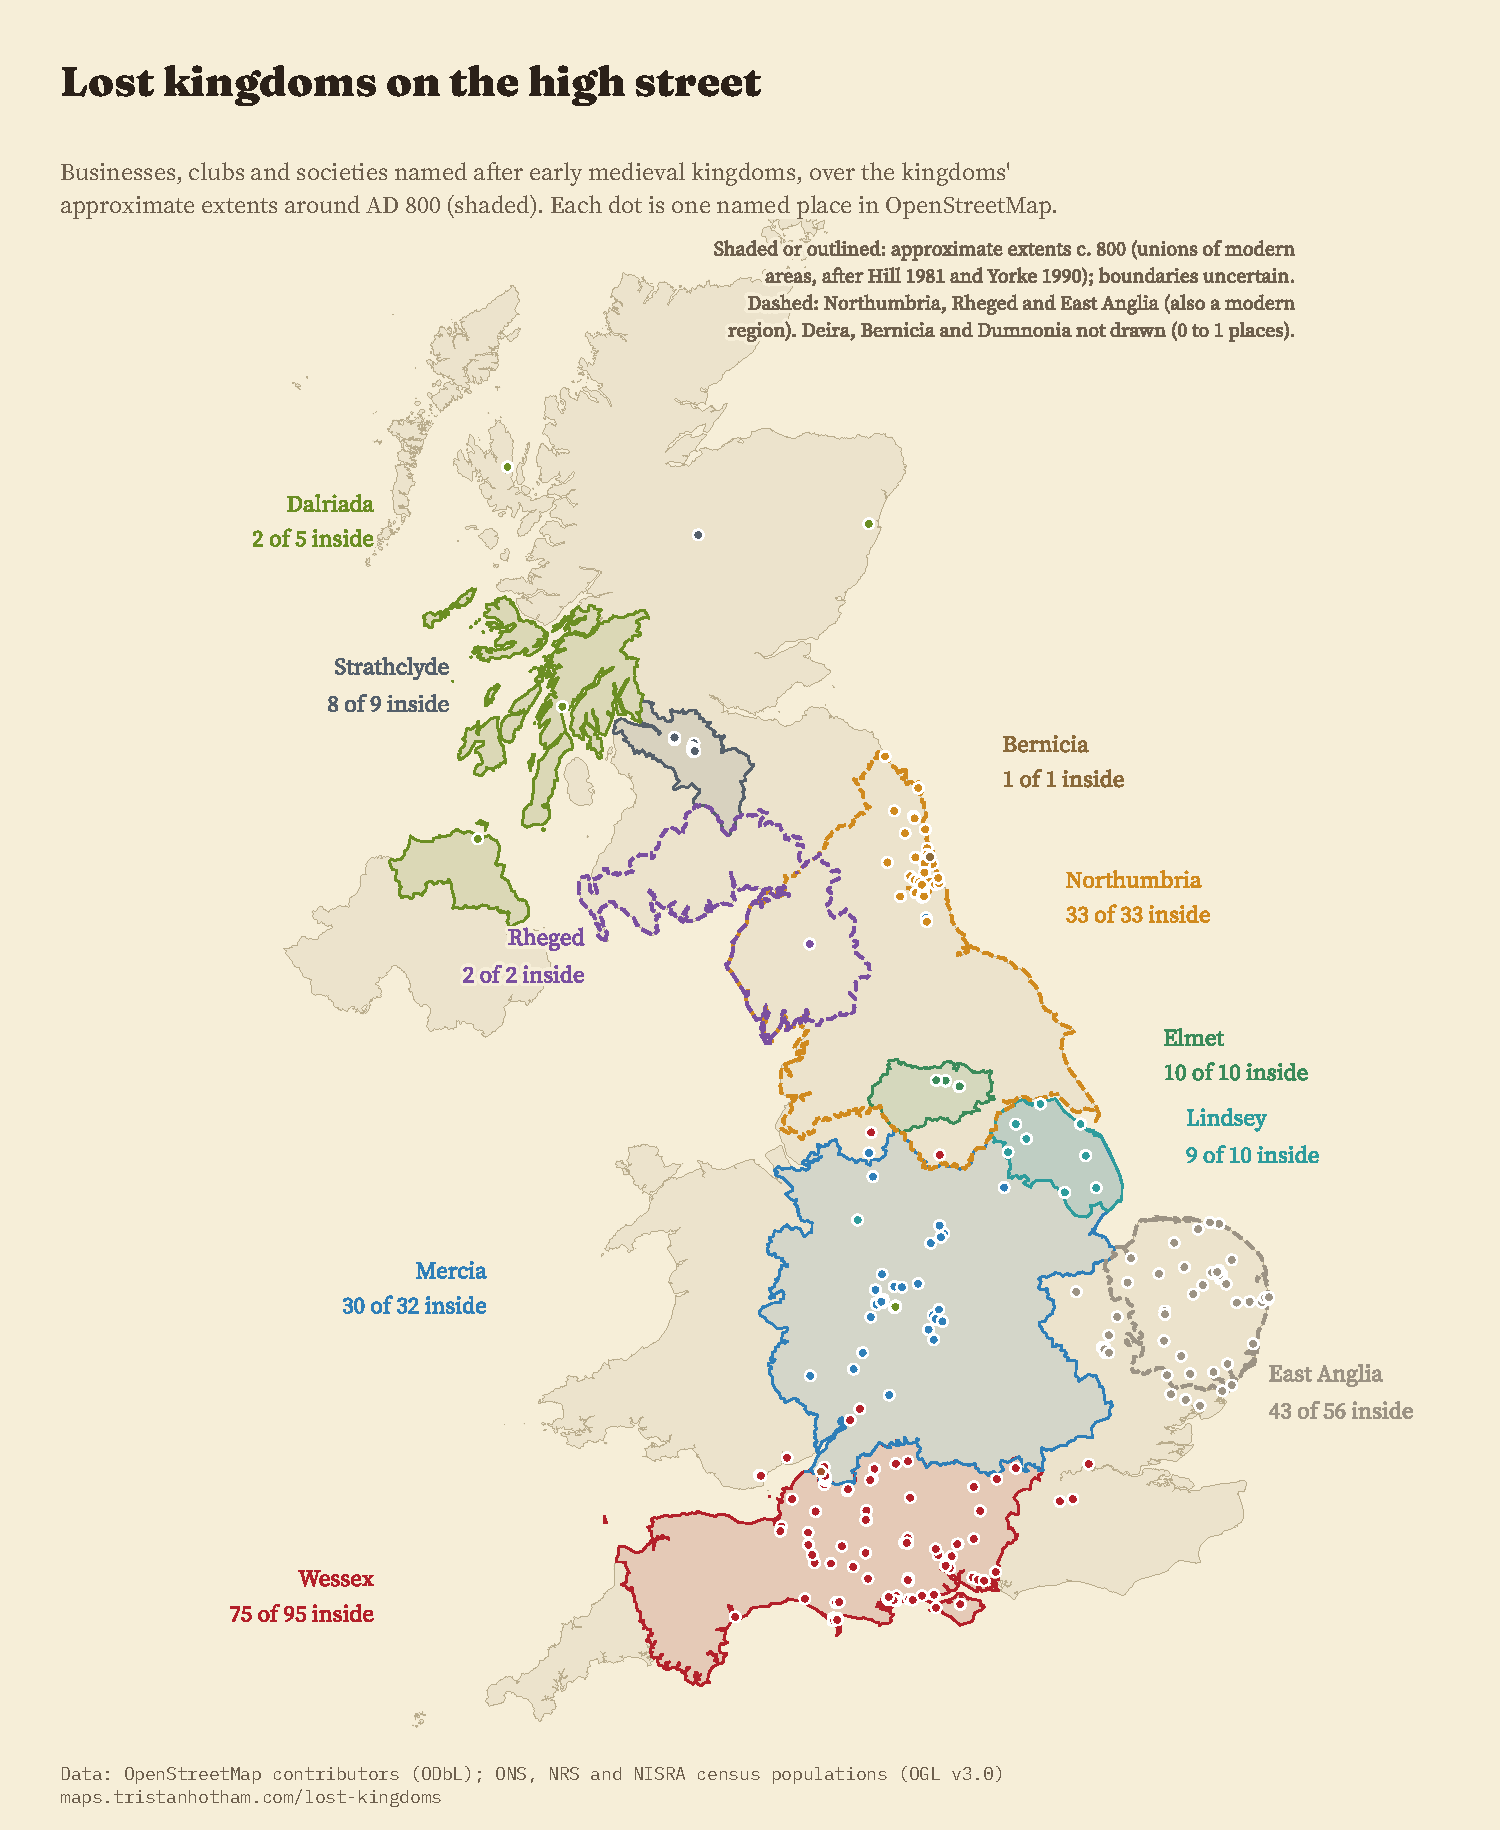
\includegraphics[width=0.86\textwidth]{f_map.pdf}\caption{Businesses and voluntary bodies named after early medieval kingdoms, over the kingdoms' approximate main extents (around AD 800). Deira, Bernicia and Dumnonia extents are not drawn (0 to 1 features). Sources: OpenStreetMap contributors (ODbL); extents after \citet{hill1981} and \citet{yorke1990}.}\label{fig:map}\end{figure}

\subsection{Baseline}
If names ignored the kingdoms, the share of a name's features inside an extent would equal the share of whatever generates businesses there. I use usual residents as the baseline: Census 2021 for England, Wales and Northern Ireland and Scotland's Census 2022, by areal unit (66,940,612 residents in all), as compiled for an earlier study \citep{hotham2026faith,ons2023}. A check uses land area instead.

\section{Research design}\label{sec:design}
The design was written in an analysis plan (\texttt{NOTES.md}) before any feature was located against any extent. At that point I had seen only the raw hit counts per word, which showed the need for whole-word matching and for reading the matches.

\textbf{Unit and outcome.} The unit is a curated named feature; the outcome is whether it lies inside the main extent of the kingdom it names. The main sample is the private class.

\textbf{H1 (tracking).} For each name $k$, private features are more common per resident inside the main extent than outside. The estimand is the rate ratio
\[ RR_k = \frac{n^{in}_k / P^{in}_k}{n^{out}_k / P^{out}_k}, \]
where $n$ counts features and $P$ residents. Because the share inside is $s_k = n^{in}_k/n_k$ and the residents' share is $b_k$, $RR_k$ is also the odds ratio $[s_k/(1-s_k)]/[b_k/(1-b_k)]$. Its 95\% interval comes from a cluster bootstrap over brands (2,000 draws), so that a chain counts as one naming decision \citep{efron1993,cameron2008}; when every feature of a name is on one side the bootstrap is degenerate and I report the Wilson bound on the share carried to the rate ratio scale. Pooled across names, I estimate a Poisson regression of feature counts by name and areal unit,
\[ E[y_{ku}] = \exp(\alpha_k + \log P_u + \beta \cdot \text{inside}_{ku}), \]
with name fixed effects, a log-population offset and standard errors clustered by local authority \citep{santos2006,cameron2015}; $\exp(\beta)$ is the pooled rate ratio. Names with fewer than 20 private features are described, not tested; the tested names are therefore Wessex, Mercia and Northumbria. East Anglia is reported separately as a modern-region comparison.

\textbf{H2 (distance decay).} Outside the extent, density per resident falls with distance from its edge: the same Poisson model over units outside each extent with distance in units of 100 km.

\textbf{H3 (private and public).} Public bodies' names lie inside the extent more often than private names, because public bodies serve defined territories. Logit of inside on a public indicator with name fixed effects, errors clustered by brand, among the tested names; a linear probability model across all names as a check.

\textbf{H4 (which names travel).} Names compared on share inside, distance and rate ratio; exploratory.

\textbf{Checks.} Placebo P1 measures each tested name against every other kingdom's main extent that does not overlap its own, among units outside its own extent; any concentration there would point to coverage or population artefacts. Robustness: R1 wide and R2 core extents; R3 each brand once; R4 leaving out each English region and each nation; R5 without place-derived and ambiguous names; R6 land area as the baseline; R7 without chains of more than three features; R8 adding streets; R9 adding ``Anglia'' and ``Anglian'' without ``East'' to East Anglia. A named building and site check (R10) was added after the plan and is labelled exploratory. A result is called robust only if its interval excludes 1 in the main specification and in every check.

\section{Results}\label{sec:results}
\subsection{Kingdom names stay in their kingdoms}
Table~\ref{tab:names} and Figure~\ref{fig:share} give the results by name. For each of the three tested names, the share of businesses and voluntary bodies inside the main extent is several times the share of residents who live there. 75 of 95 Wessex names (79\%, Wilson CI 70 to 86) are inside an extent holding 10.0\% of residents, a rate ratio of 33.9 (brand bootstrap CI 19.5 to 70.7). Mercia, the largest extent with 25.6\% of residents, has 30 of 32 inside (rate ratio 43.6, CI 15.1 to 200.6). All 33 Northumbria names are inside Northumbria (Wilson CI for the share 90 to 100\%, so the rate ratio is at least 50), and all 33 are in the present-day North East region. The pooled Poisson estimate is 44.0 (CI 19.5 to 99.7; 160 features, 361 local authority clusters), and across all eleven kingdom names with any private feature it is 83.5 (CI 34.1 to 204.6). H1 is supported.

\begin{table}[tbp]\centering\footnotesize\caption{Kingdom names: businesses and voluntary bodies (private) inside the main extent, the share of UK residents there, and the rate ratio per resident inside vs outside (brand bootstrap 95\% CI; for names with every feature inside, the Wilson lower bound). Public bodies and streets: number and \% inside. Tested names in bold.}\label{tab:names}\setlength{\tabcolsep}{3.5pt}\begin{tabular}{lrrrlrlll}\toprule Name & Private & Brands & Inside & \% inside [CI] & \% residents & Rate ratio [CI] & Public & Streets\\\midrule
\textbf{Wessex} & 95 & 74 & 75 & 79 [70, 86] & 10.0 & 33.9 [19.5, 70.7] & 15 (93\%) & 130 (52\%)\\
\textbf{Mercia} & 32 & 28 & 30 & 94 [80, 98] & 25.6 & 43.6 [15.1, 200.6] & 19 (79\%) & 74 (68\%)\\
\textbf{Northumbria} & 33 & 31 & 33 & 100 [90, 100] & 14.7 & $\geq$50 & 21 (95\%) & 16 (38\%)\\
Elmet & 10 & 10 & 10 & 100 [72, 100] & 3.7 &  & 5 (100\%) & 21 (100\%)\\
Lindsey & 10 & 7 & 9 & 90 [60, 98] & 1.0 &  & 12 (100\%) & 61 (18\%)\\
Strathclyde & 9 & 6 & 8 & 89 [56, 98] & 2.8 &  & 9 (100\%) & 12 (58\%)\\
Dalriada & 5 & 5 & 2 & 40 [12, 77] & 0.5 &  & 5 (60\%) & 14 (57\%)\\
Rheged & 2 & 2 & 2 & 100 [34, 100] & 1.0 &  & 0 & 1 (100\%)\\
Bernicia & 1 & 1 & 1 & 100 [21, 100] & 5.1 &  & 0 & 2 (50\%)\\
Dumnonia & 1 & 1 & 0 & 0 [0, 79] & 2.9 &  & 0 & 0\\
Deira & 0 & 0 & 0 & n/a & 2.6 &  & 0 & 4 (50\%)\\
\midrule
East Anglia & 56 & 24 & 43 & 77 [64, 86] & 2.5 &  & 7 (71\%) & 1 (100\%)\\
\bottomrule\end{tabular}\end{table}

\begin{figure}[tbp]\centering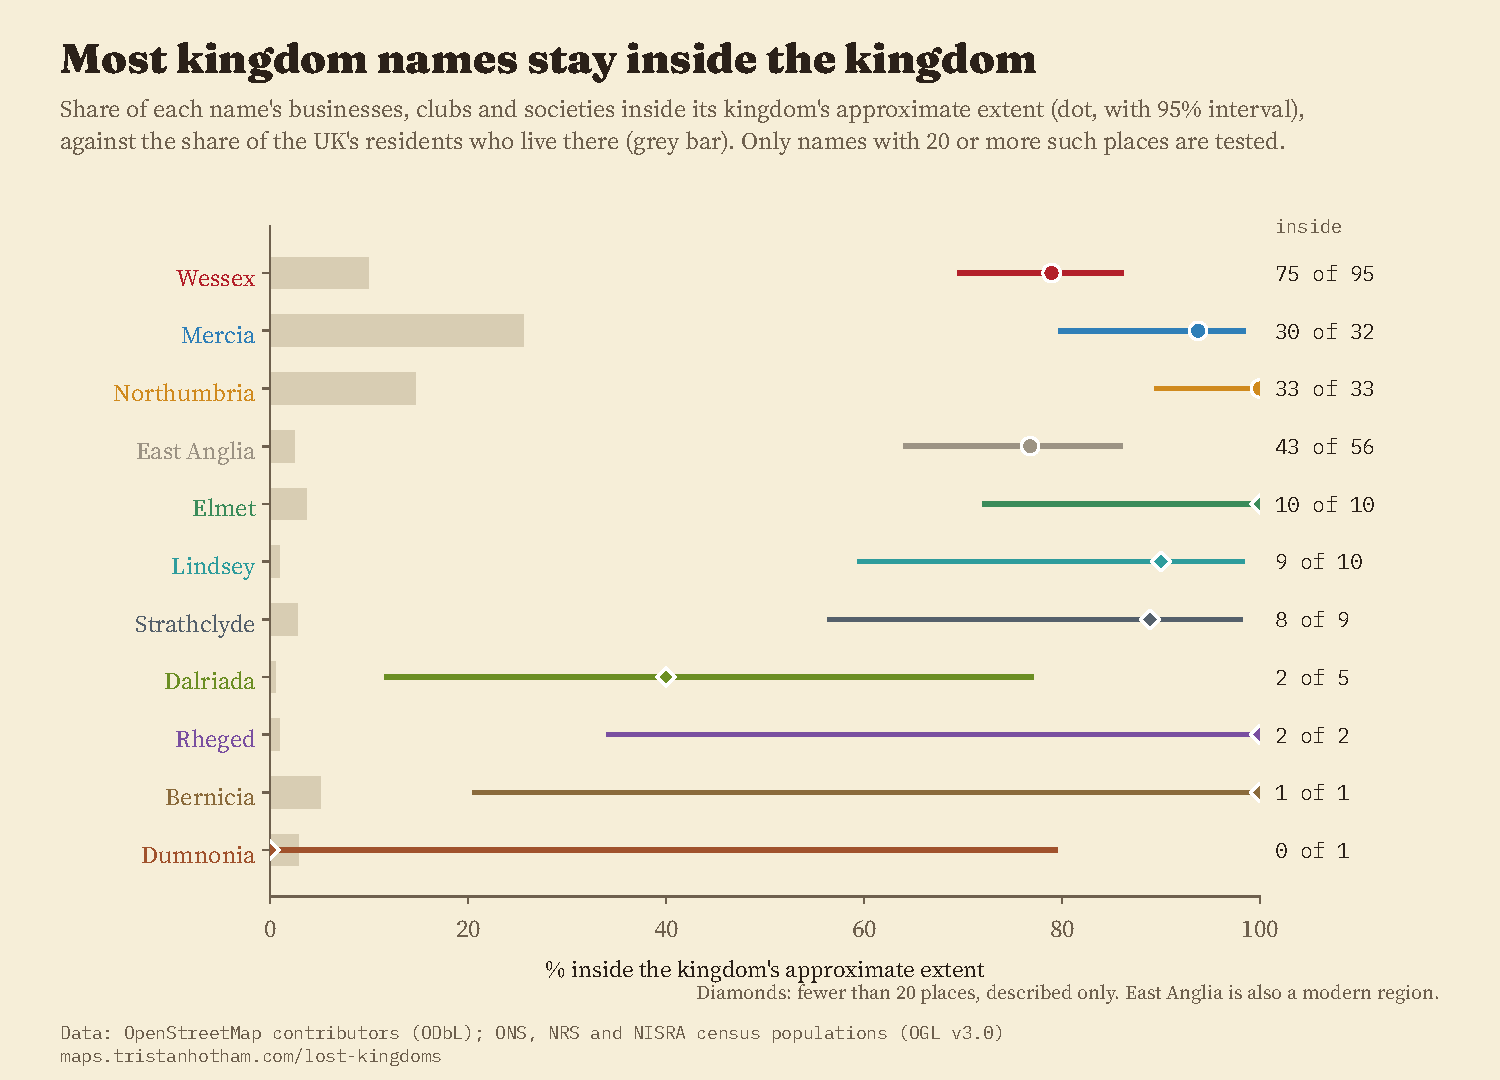
\includegraphics[width=0.9\textwidth]{f_share.pdf}\caption{Share of each name's businesses and voluntary bodies inside its kingdom's main extent (95\% Wilson interval) against the share of UK residents living there. Diamonds: fewer than 20 features, described only.}\label{fig:share}\end{figure}

The smaller kingdoms point the same way, though with few cases each. All 10 Elmet names are inside the Elmet extent around Leeds and Selby, but 6 of them come from Sherburn in Elmet, Barwick in Elmet or Elmete in Leeds. Lindsey has 9 of 10 inside and Strathclyde 8 of 9. Rheged has only 2 private features, both at the Rheged visitor centre near Penrith, inside the extent. Dalriada is the one name that is not mostly inside: 2 of 5, with the others in the Highlands, Aberdeen and Birmingham. Deira, Bernicia and Dumnonia have at most one private feature each. East Anglia, which is a modern region as well as a kingdom, has 43 of 56 features in Norfolk and Suffolk and all of them within the wider modern sense that adds Cambridgeshire and Essex; its brands are fewer (24), because one hospice charity has many shops.


\subsection{The cases, read one by one}
Because every feature was read, the numbers can be set beside what the names are. The Wessex names are a cross-section of local commerce: car dealers and garages, pharmacies, photographic and picture-framing shops, dry cleaners, locksmiths, solicitors, a funeral director, an angling shop, two pubs called the King of Wessex, a cancer charity and its shops, an archaeology charity, a cave club and a squash club. Very few are national brands; the largest are a pharmacy group, a photographic shop chain and a car dealership group, each with a handful of branches. The Mercia names are similar but fewer: carpet shops, a cycle maker, estate and letting agents, a newsagent, a marina, two pubs called the Earl of Mercia, a property company and a scout group under the West Mercia name. The Northumbria names lean towards food and gifts (heritage meats, a hamper shop, a foodhall, a jeweller, gift shops called Pride of Northumbria and Taste of Northumbria) and towards clubs (gliding, cycle speedway, amateur radio), which may suggest that in the North East the name carries a sense of regional produce and pride rather than of antiquity.

The small kingdoms are a different kind of evidence. Elmet's ten features are a fish and chip shop, a restaurant, a dental practice and a social club in the Selby and Leeds area, and six that take their name from Sherburn in Elmet, Barwick in Elmet or Elmete; the kingdom's name survives commercially only where it survives in place names, which is itself a finding about how such names persist. Lindsey's private and public features are dominated by bodies named after the Parts of Lindsey and the modern districts (two drainage boards, a hospice and its shops, an Age UK branch, a blind society). Strathclyde's are mostly named after Strathclyde Park, the business park or the university, all of which take the name from the valley and the later region rather than directly from the kingdom. Most of the Dalriada names in Northern Ireland are inside the north Antrim part of the extent, and the three private features outside it are a guesthouse, a sports ground and a trustee firm's office, a mixture that looks like individual choices rather than a pattern. Rheged's two features both belong to the Rheged visitor centre near Penrith, which is named after the kingdom.

\subsection{Where the names that leave go}
Figure~\ref{fig:wessex} shows the 20 Wessex names outside the main extent. 14 are within 25 km of the edge: 7 in Bristol, which the main extent leaves to Mercia because it lies north of the Avon, and 4 car dealerships of one group in Cardiff and Newport across the Severn. 9 of the 20 are inside the wide extent. The furthest, in Oldham, is 204 km from the extent. Appendix Table~\ref{tab:out} lists every business and public body outside its kingdom's main extent. Of Mercia's two outsiders, one is a garage in Stockport, just north of the Cheshire boundary; the other is in County Durham.

\begin{figure}[tbp]\centering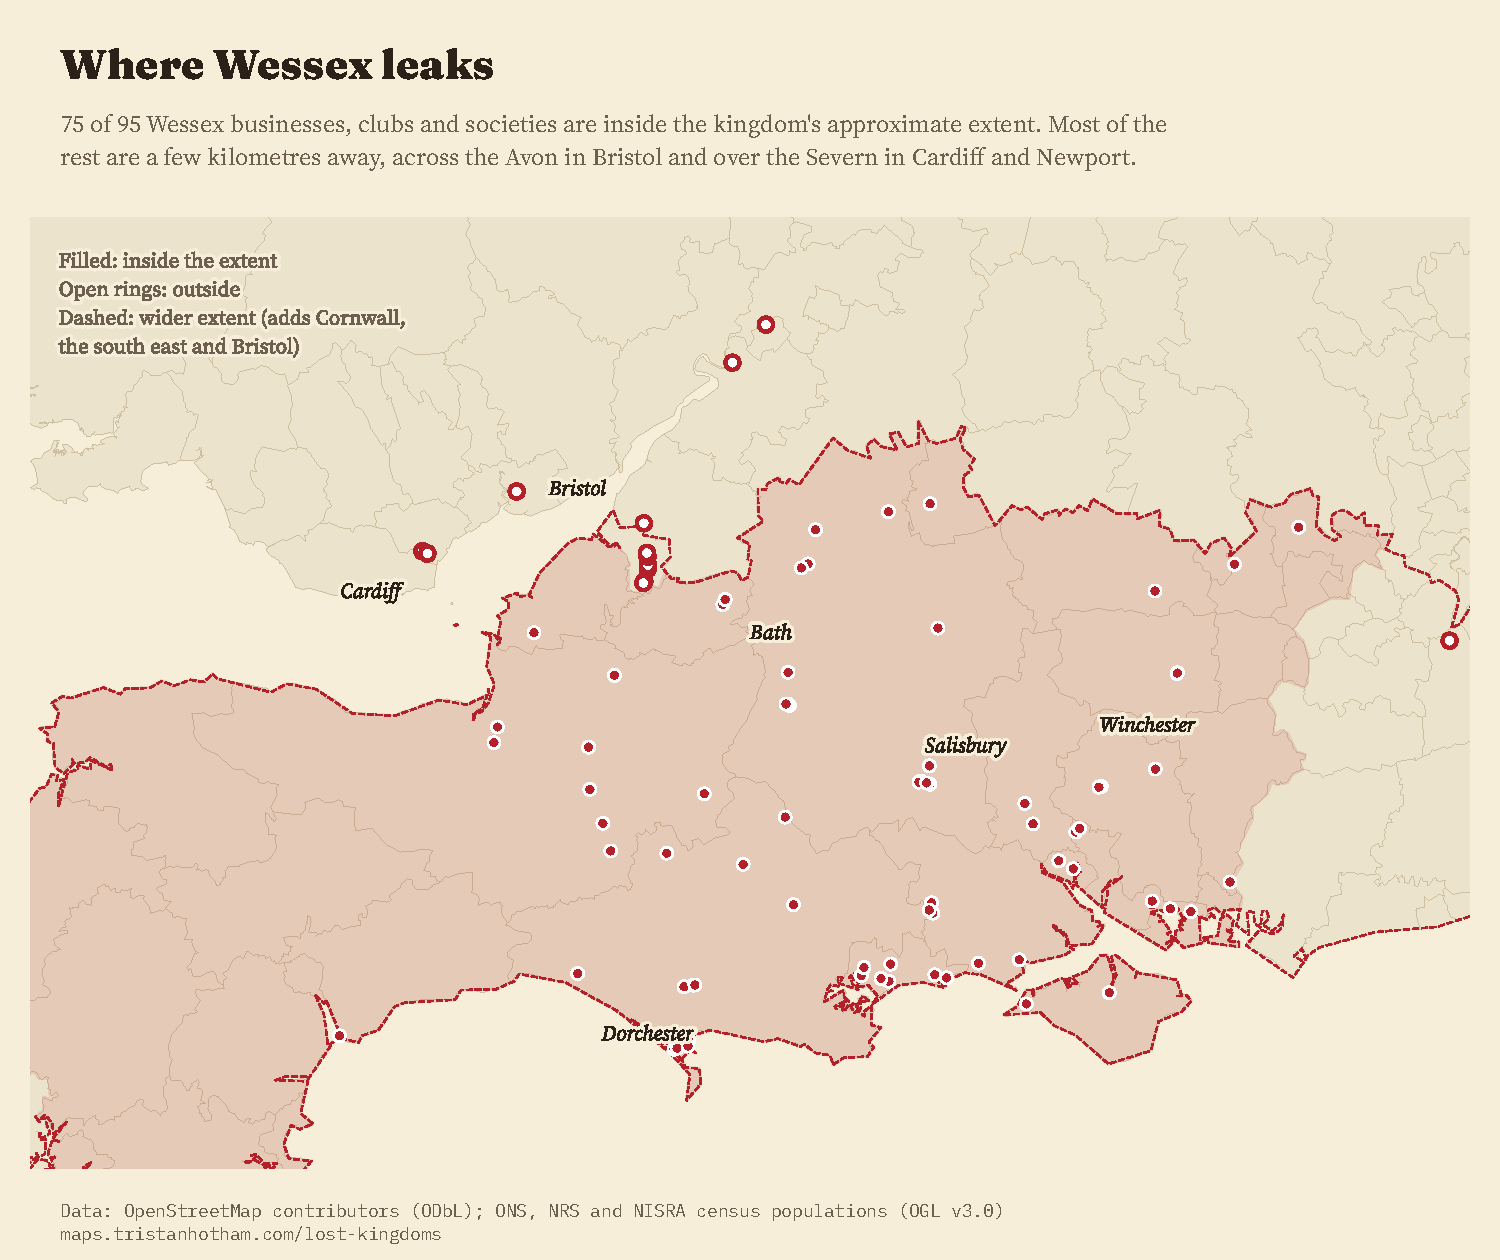
\includegraphics[width=0.9\textwidth]{f_wessex.pdf}\caption{Wessex businesses and voluntary bodies inside (filled) and outside (rings) the main extent; dashed line, the wide extent.}\label{fig:wessex}\end{figure}

H2 asked whether density falls with distance outside the extent. It can be estimated only for Wessex, the one tested name with more than a handful of features outside (Mercia has 2, Northumbria none). The Wessex estimate is a rate ratio of 0.10 per 100 km (CI 0.01 to 1.85; 20 features outside), too imprecise to support or reject H2. Figure~\ref{fig:bands} shows why: almost all of the fall happens at the edge. Pooling the three tested names, there are 4.10 kingdom-named businesses per million residents inside the extents, 0.48 within 25 km outside and 0.09 at 25 to 50 km. The pattern looks less like a gradual decay than a step at the boundary with a short spillover.

\begin{figure}[tbp]\centering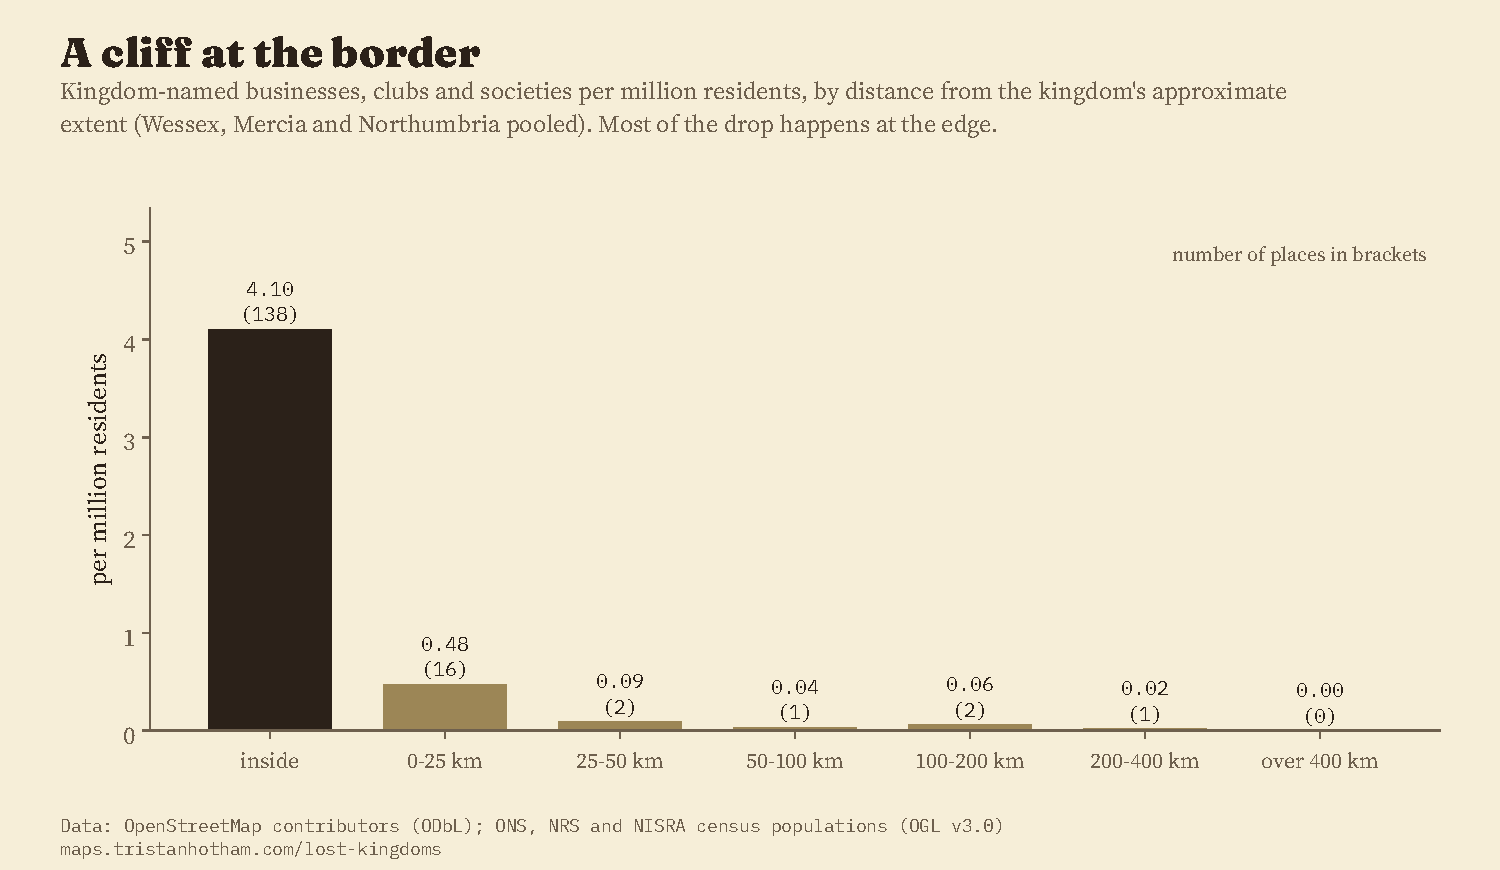
\includegraphics[width=0.9\textwidth]{f_bands.pdf}\caption{Kingdom-named businesses and voluntary bodies per million residents by distance from the main extent, Wessex, Mercia and Northumbria pooled (number of features in brackets).}\label{fig:bands}\end{figure}

\subsection{Businesses, public bodies and streets}
H3 is not supported. Among the tested names, 89\% of public bodies and 86\% of businesses and voluntary bodies are inside their kingdom's extent; the odds ratio for public bodies is 0.87 (CI 0.29 to 2.60; 215 features, 55 public), and the linear probability model over all names gives a difference of 1.9 percentage points (CI $-$6.5 to 10.3). Both kinds of name are local. The public bodies outside are instructive: a Northumbria University campus in London, Mercian Regiment buildings in Wiltshire, a Wessex reserve training camp in South Gloucestershire. They sit where the institutions have sites.

Streets behave differently (Figure~\ref{fig:types}). Only 52\% of the 335 streets named after the eleven kingdoms are inside the main extent, against 86\% of private names across all the kingdoms. The pooled rate ratio for streets is 7.9 (CI 5.4 to 11.6): streets still concentrate in their kingdom, but far less, and outside the extent they show the gradual decay that businesses do not, 0.64 per 100 km (CI 0.50 to 0.80). This exploratory comparison fits the way streets are named in Britain, from lists of themed names proposed by developers and approved by councils, in which a grand historical name can be chosen for its sound. A Wessex Close in the Midlands costs its namer nothing; a Wessex Garage there would tell its customers little about where it is.

\begin{figure}[tbp]\centering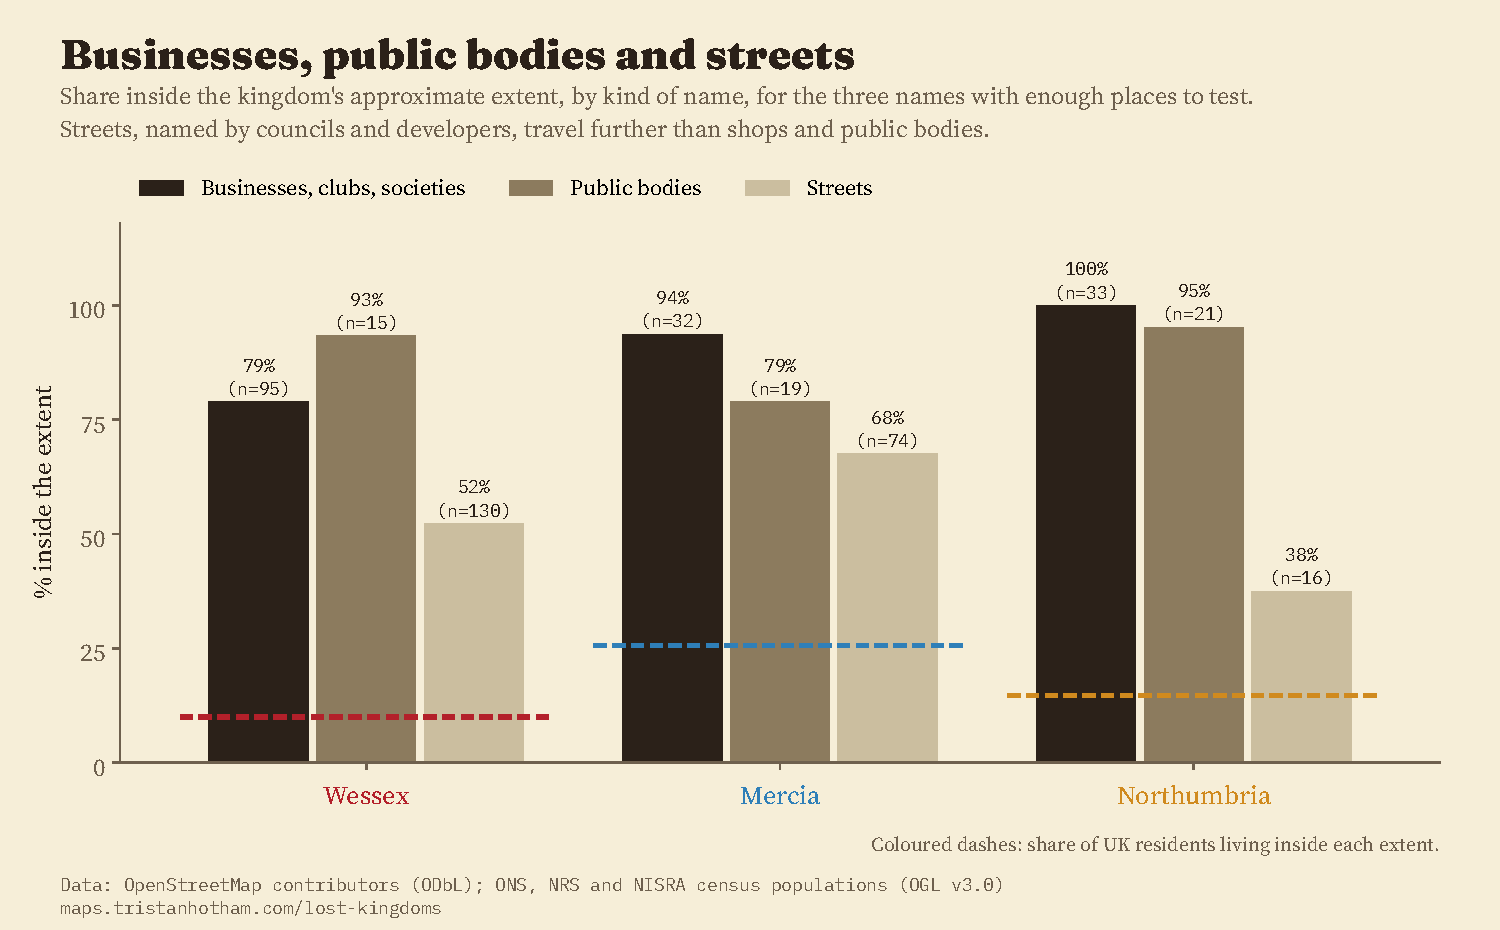
\includegraphics[width=0.9\textwidth]{f_types.pdf}\caption{Share inside the main extent by kind of name, for the three tested names. Dashes: share of UK residents inside each extent.}\label{fig:types}\end{figure}

\subsection{Which names travelled furthest}
Among the tested names, Wessex is the least confined (79\% inside), then Mercia (94\%) and Northumbria (100\%). The intervals overlap, and the ordering partly reflects geography: Wessex's main extent has a long land boundary next to large cities (Bristol, and Cardiff and Newport across the Severn), while Northumbria's is bounded by the sea, Scotland and the thinly populated Pennines. Measured by the median distance of features from the kingdom's centre, Wessex names are 71 km from Winchester, Mercia names 30 km from Tamworth and Northumbria names 60 km from Bamburgh. Hardy's revival has not produced a footloose brand: four in five Wessex names are inside Wessex. Among the small names, only Dalriada has travelled, and its handful of cases cannot say why.

\section{Placebo and robustness}\label{sec:robust}
\textbf{Placebo.} Measured against the main extents of other kingdoms that do not overlap their own, among units outside their own extent, the tested names show no concentration: the pooled rate ratio is 0.97 (CI 0.51 to 1.83; 27 name and extent pairs, 14 features inside a wrong extent). Whatever produces the concentration is specific to each name's own kingdom; it is not a general tendency of OpenStreetMap businesses to be mapped in some regions rather than others.

\textbf{Robustness.} Table~\ref{tab:robust} and Figure~\ref{fig:robust} report every planned check. The pooled rate ratio for the tested names ranges from 14.5 to 66.2 across the 19 checks, and its interval excludes 1 in all of them; the same holds for the all-names pooled model (25.0 to 139.7) and for Wessex alone (15.8 to 51.4). The largest change comes from adding streets (R8), which lowers the estimate as Section~\ref{sec:results} would predict. Leaving out the South West, which removes most of Wessex, raises it. Counting each brand once, or dropping chains, changes little, so the result is not a few chains. Using land area instead of residents as the baseline raises the estimate slightly. Dropping place-derived and ambiguous names does not affect the tested names (none of their features are flagged) and lowers the all-names estimate to 62.0. East Anglia with ``Anglia'' and ``Anglian'' names added (R9) has 62\% inside Norfolk and Suffolk, against 77\% for ``East Anglia'' alone: the shorter forms travel further, as expected of names used by regional companies such as the water utility and a university whose territories extend beyond the two counties.

\begin{table}[tbp]\centering\scriptsize\caption{Robustness: rate ratio inside vs outside per resident (Poisson with name fixed effects and a log-population offset, R6 log-area; 95\% CI clustered by local authority) for the three tested names pooled, all eleven kingdom names pooled, and Wessex alone. N = features in the tested-names model.}\label{tab:robust}\setlength{\tabcolsep}{3pt}\begin{tabular}{p{6.2cm}rlll}\toprule Check & N & Tested names & All names & Wessex\\\midrule
\multicolumn{4}{l}{\textit{Main}}\\
\quad Main specification & 160 & 44.0 [19.5, 99.7] & 83.5 [34.1, 204.6] & 33.9 [13.9, 82.9]\\
\multicolumn{4}{l}{\textit{Extent}}\\
\quad R1 wide extents & 160 & 39.8 [18.4, 86.4] & 80.8 [38.9, 167.6] & 33.3 [14.1, 78.7]\\
\quad R2 core extents & 160 & 48.3 [25.0, 93.5] & 59.0 [30.1, 115.7] & 38.1 [18.2, 79.4]\\
\multicolumn{4}{l}{\textit{Counting}}\\
\quad R3 each brand once & 133 & 54.2 [23.0, 127.7] & 96.1 [39.6, 233.1] & 42.4 [16.3, 110.6]\\
\multicolumn{4}{l}{\textit{Leave one region out}}\\
\quad R4 without East Midlands & 155 & 41.5 [18.3, 93.9] & 70.6 [28.6, 174.6] & 31.1 [12.7, 76.1]\\
\quad R4 without East of England & 160 & 39.9 [17.7, 90.2] & 75.6 [30.9, 184.9] & 30.3 [12.4, 74.1]\\
\quad R4 without London & 159 & 39.2 [16.9, 90.9] & 75.0 [29.9, 188.1] & 30.5 [12.1, 76.8]\\
\quad R4 without North East & 126 & 35.1 [15.2, 81.2] & 74.0 [28.5, 192.4] & 32.4 [13.3, 79.2]\\
\quad R4 without North West & 157 & 45.1 [18.5, 109.4] & 79.1 [31.2, 200.4] & 31.3 [12.4, 78.9]\\
\quad R4 without Northern Ireland & 160 & 42.6 [18.8, 96.5] & 81.7 [32.1, 207.9] & 32.8 [13.4, 80.3]\\
\quad R4 without Scotland & 160 & 39.9 [17.7, 90.3] & 70.0 [26.3, 186.3] & 30.8 [12.6, 75.3]\\
\quad R4 without South East & 132 & 48.9 [20.1, 118.9] & 88.1 [35.9, 216.2] & 39.5 [14.1, 110.6]\\
\quad R4 without South West & 100 & 66.2 [30.7, 142.6] & 139.7 [68.6, 284.8] & 51.4 [21.4, 123.6]\\
\quad R4 without Wales & 156 & 50.8 [20.5, 125.9] & 96.7 [36.9, 253.6] & 40.2 [14.7, 110.1]\\
\quad R4 without West Midlands & 136 & 39.1 [16.6, 92.1] & 80.2 [30.2, 213.4] & 32.2 [12.7, 81.1]\\
\quad R4 without Yorkshire and The Humber & 159 & 50.9 [20.4, 127.1] & 74.8 [28.3, 197.4] & 32.4 [12.8, 81.9]\\
\multicolumn{4}{l}{\textit{Names}}\\
\quad R5 without place-derived and ambiguous names & 160 & 44.0 [19.5, 99.7] & 62.0 [25.6, 150.5] & 33.9 [13.9, 82.9]\\
\multicolumn{4}{l}{\textit{Baseline}}\\
\quad R6 per square kilometre, not per resident & 160 & 50.6 [21.5, 118.9] & 89.7 [36.0, 223.4] & 37.1 [14.5, 94.5]\\
\multicolumn{4}{l}{\textit{Counting}}\\
\quad R7 without chains (brands with more than 3 features) & 146 & 38.4 [16.9, 87.4] & 72.5 [28.7, 183.6] & 27.6 [11.2, 67.6]\\
\multicolumn{4}{l}{\textit{Classes}}\\
\quad R8 private names plus streets & 380 & 14.5 [9.5, 22.1] & 25.0 [16.4, 38.1] & 15.8 [9.7, 25.7]\\
\quad R10 private names plus named buildings and sites (exploratory) & 200 & 37.9 [19.9, 72.1] & 70.1 [35.9, 136.9] & 29.0 [14.4, 58.8]\\
\quad Public bodies only (H3 comparison) & 55 & 45.5 [13.9, 148.8] & 263.4 [86.5, 802.6] & 126.5 [16.3, 979.4]\\
\bottomrule\end{tabular}\end{table}

\begin{figure}[tbp]\centering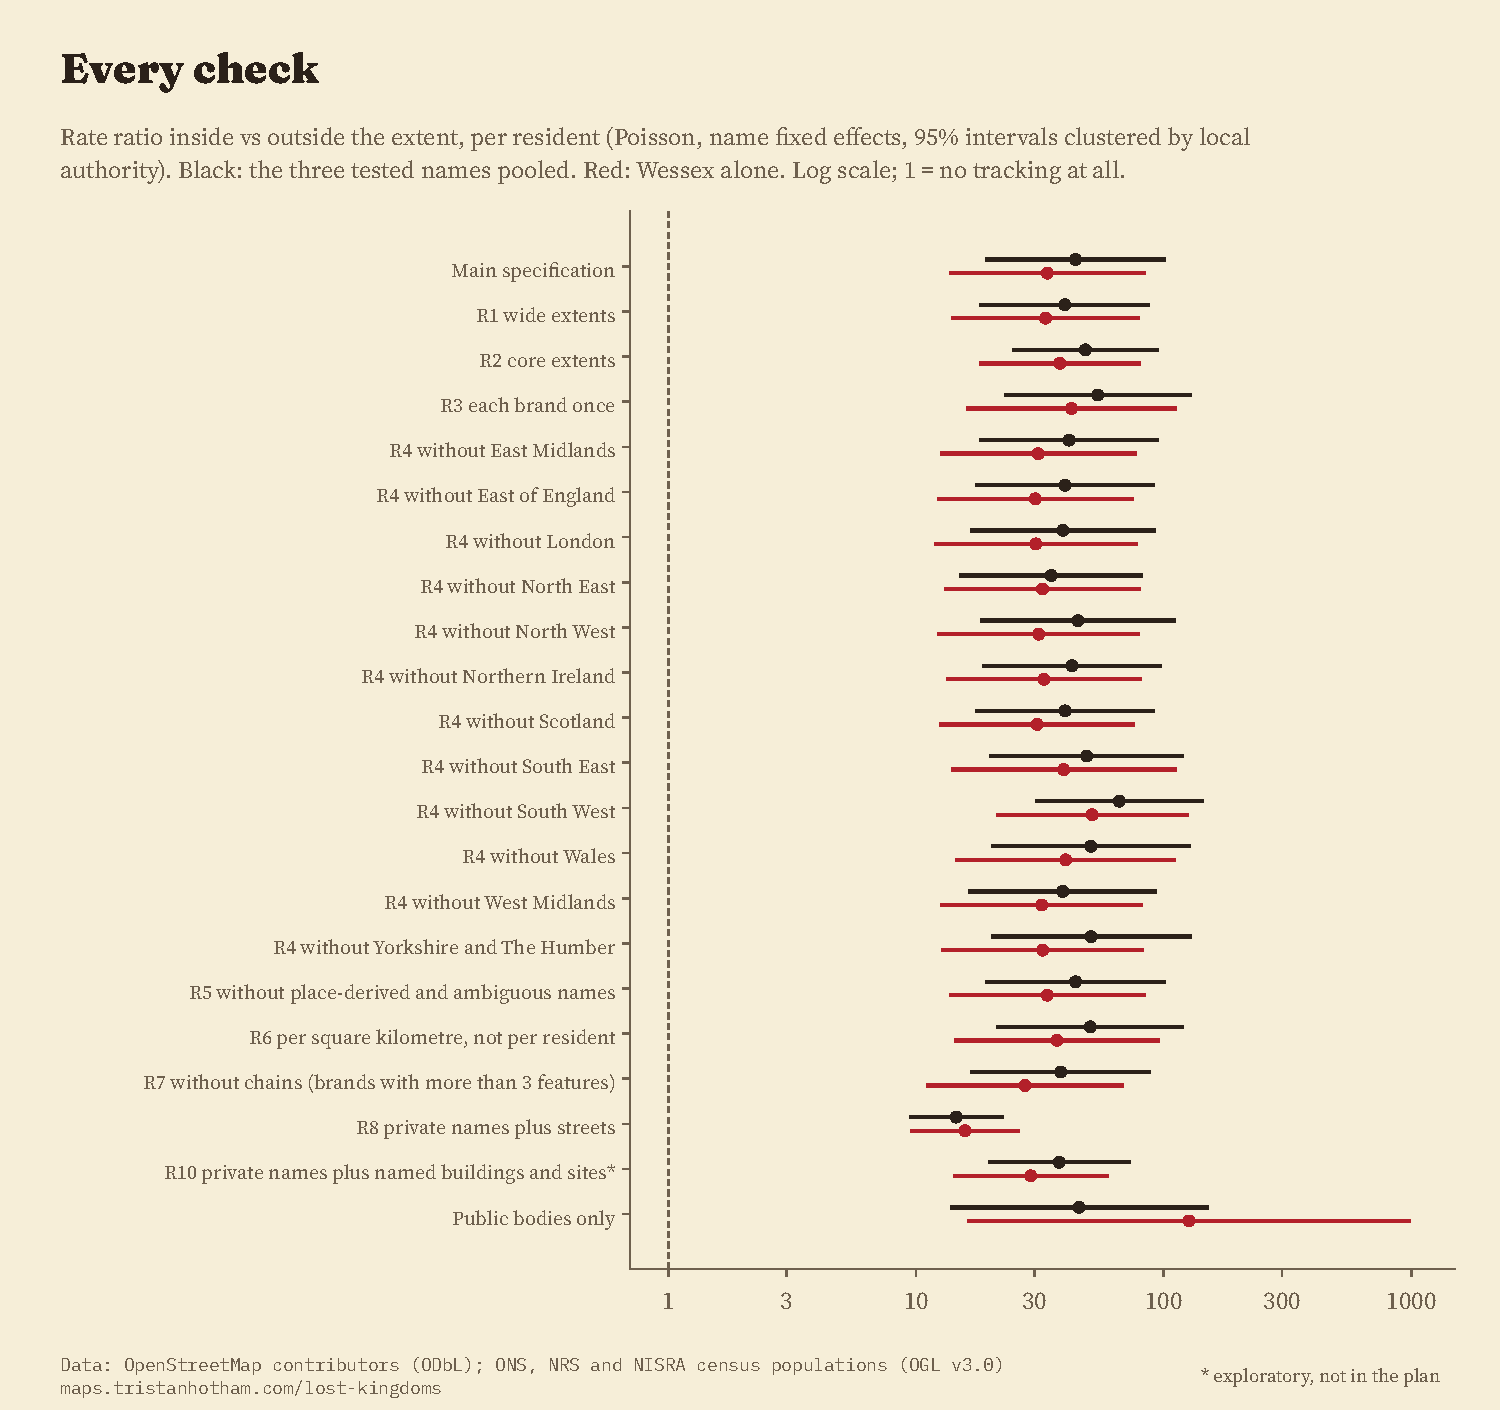
\includegraphics[width=0.92\textwidth]{f_robust.pdf}\caption{Every check: pooled rate ratio for the tested names (black) and Wessex alone (red), with 95\% intervals clustered by local authority; log scale.}\label{fig:robust}\end{figure}

\section{Discussion}\label{sec:disc}
\subsection{Interpretation}
The names of kingdoms that ended more than a thousand years ago are used today almost entirely inside the areas those kingdoms covered. This is not what one would expect of purely romantic or literary names. It suggests that, for the people who choose them, the names work as regional labels: a Northumbrian butcher or a Mercian cycle maker is saying where it is. In \citeauthor{paasi1986}'s terms, the kingdoms have kept, or regained, a symbolic shape tied to a territorial one, even without an institutional shape of their own \citep{paasi1986,paasi2003}.

Two mechanisms are consistent with the result, and the data cannot separate them. In the first, long continuity: the names never wholly left local use, surviving in places such as Sherburn in Elmet and Kirton in Lindsey, in the antiquarian and educational culture of each region, and in local histories. In the second, modern institutional revival: the names were re-attached to regions by police forces, utilities, regiments, broadcasters and universities, and businesses followed. The Northumbria result fits the second especially well: every Northumbria business is in the present-day North East, where Northumbria Police, Northumbrian Water and Northumbria University operate, and none is in Yorkshire, which was as much a part of the kingdom. In this reading, the modern name tracks the modern institutions, and the institutions happen to sit inside a historical extent drawn generously enough to contain them. The same may be true of Wessex: inside the main extent its business names are most numerous in Dorset (22) and Hampshire (21), and Dorset is Hardy's home county.

The result for streets is a useful contrast. Streets are named by a different process, in which developers propose and councils approve, often from themed lists. Kingdom names on streets are much less local, and they decay gradually with distance, which suggests that for a street name the kingdom is decoration rather than location. Commercial names are commodities in \citet{lightyoung2015}'s sense, but the commodity a regional name sells is the region.


\subsection{What the extents can and cannot carry}
The extents deserve a further word, because the whole design rests on them. They are not maps of where any early medieval king ruled on any given day; they are a reproducible statement of where most historians would place each kingdom's centre of gravity around AD 800, expressed in modern units. Three features of the result make it unlikely that the drawing of the lines drives it. First, the concentration is so strong that even the widest extents, which add whole counties of doubtful membership, and the narrowest, which keep only the heartlands, give rate ratios in the same range. Second, most features outside the main extents sit within a few kilometres of the edge, in places such as Bristol and Stockport whose assignment was a judgement made before the data were seen; moving the line would change the count by a handful. Third, the placebo uses the same lines for the wrong names and finds nothing. The extents are, however, much too coarse to say anything about the precise course of a boundary, or about whether, for example, Wessex names respect the Avon or the Severn as such. Those questions would need a much larger set of names and a finer treatment of the frontier zones.

There is also a sense in which the modern names define their own extents. Northumbria in present-day use means the North East, not the kingdom from the Humber to the Forth; East Anglia means a region that some would extend to Essex and Cambridgeshire; Strathclyde for many people means the council region of 1975 to 1996 rather than the kingdom. A historical extent drawn generously enough will contain the modern sense, and the results here show that the names stay within the historical extents, not that they reproduce them. The share of the historical extent that the names actually fill is another question. For Northumbria the answer is plainly that they fill only the north eastern part.

\subsection{Relation to earlier work}
Studies of street names have shown that names record political and cultural choices and can be read as data at scale \citep{azaryahu1996,alderman2000,otoperalias2018,bancilhon2021,gutierrez2022}, and that names, once given, persist through habit even after the regimes that gave them have gone \citep{lightyoung2014}. The present study adds a commercial and regional dimension. The kingdom names on businesses are not imposed by any authority; each is chosen by an owner. That such choices, made separately by 160 businesses and voluntary bodies for the three tested names, mostly stay within extents drawn from a map more than a thousand years old fits \citet{paasi2003}'s view of regional identities as continually reproduced rather than simply inherited. It also shows the value of open, map-wide data for questions that onomastics has usually approached through dictionaries and case studies.

\subsection{Limitations}
The study has clear limits. OpenStreetMap does not record every business; its coverage is uneven, and businesses with a regional name may be more or less likely to be mapped than others. The placebo and the land-area check speak against a coverage artefact producing the result, but they cannot rule out every bias. Companies House, which would give a near-complete register of company names with registered addresses, could not be reached from the workspace in which this study was built, and registered addresses are often not trading addresses anyway. The source file has exactly 7,500 rows, which could mean a query limit. It is sorted by OpenStreetMap identifier, so a limit would have cut only the identifiers that sort last. A second export without a limit, with exact keywords (5,835 rows, 1,775 kingdom-name objects), stopped on a time-out before it reached point features, so it cannot prove completeness; but every kingdom-name object in it is already in the main file (0 missing), and none of its objects sorts after the main file's last row.

The kingdom extents are approximations of uncertain historical boundaries drawn with modern administrative lines. The three versions bracket some of this uncertainty, and the result holds in all three, but a different scholar would draw different lines. The sample is small: 198 private features for the eleven kingdom names, of which most belong to three names, so the smaller kingdoms can only be described. I cannot date the names, so I cannot say whether they predate or follow any revival. Finally, the design is observational. A business named Wessex in Dorset may have chosen the name because it is in Wessex, or for some other reason that happens to be commoner in Dorset.

\subsection{Further work}
The design extends naturally to other historical regions (the historic counties, the Danelaw, the Welsh kingdoms) and to registers that include company incorporation dates, which would allow the timing of revivals to be studied: whether new Mercia names cluster after the creation of West Mercia Police, for example, or new Wessex names after the Wessex novels. A survey of business owners would get closer to why the names are chosen.

\section{Conclusion}\label{sec:conc}
The early medieval kingdoms are gone, but their names are still local. Businesses, clubs and societies named after Wessex, Mercia and Northumbria are found mostly inside the approximate extents of those kingdoms, at 44 times the rate per resident found outside, and the names that leave mostly stop just over the boundary. Public bodies are as local as businesses; streets are not. Whatever the route by which the names came back into use, they came back to the places they describe.

\section*{Data availability}
Data and code: Zenodo DOI https://doi.org/10.5281/zenodo.24104340. Interactive map: \url{https://maps.tristanhotham.com/lost-kingdoms/}. Repository: \url{https://github.com/Tristan-Hotham/lost-kingdoms}. Derived data from OpenStreetMap are under the Open Database Licence 1.0; census populations under the Open Government Licence v3.0.

\section*{AI statement}
I wrote the text, with drafting and editing assistance from Claude (Anthropic), which also helped prepare the analysis code. I reviewed and checked all text and results.

\begin{thebibliography}{99}
\bibitem[Alderman(2000)]{alderman2000} Alderman, D. H. (2000) A street fit for a King: naming places and commemoration in the American South. \textit{The Professional Geographer} 52(4), 672 to 684. doi:10.1111/0033-0124.00256.
\bibitem[Azaryahu(1996)]{azaryahu1996} Azaryahu, M. (1996) The power of commemorative street names. \textit{Environment and Planning D: Society and Space} 14(3), 311 to 330. doi:10.1068/d140311.
\bibitem[Bancilhon et al.(2021)]{bancilhon2021} Bancilhon, M., Constantinides, M., Bogucka, E. P., Aiello, L. M. and Quercia, D. (2021) Streetonomics: quantifying culture using street names. \textit{PLoS ONE} 16(6), e0252869. doi:10.1371/journal.pone.0252869.
\bibitem[Bassett(1989)]{bassett1989} Bassett, S. (ed.) (1989) \textit{The Origins of Anglo-Saxon Kingdoms}. London: Leicester University Press.
\bibitem[Bast and Buchhold(2017)]{bast2017} Bast, H. and Buchhold, B. (2017) QLever: a query engine for efficient SPARQL+Text search. In \textit{Proceedings of the 26th ACM International Conference on Information and Knowledge Management (CIKM 2017)}, 647 to 656. doi:10.1145/3132847.3132921.
\bibitem[Bast et al.(2021)]{bast2021} Bast, H., Brosi, P., Kalmbach, J. and Lehmann, A. (2021) An efficient RDF converter and SPARQL endpoint for the complete OpenStreetMap data. In \textit{Proceedings of the 29th International Conference on Advances in Geographic Information Systems (SIGSPATIAL 2021)}. doi:10.1145/3474717.3484256.
\bibitem[Brown and Farr(2001)]{brownfarr2001} Brown, M. P. and Farr, C. A. (eds) (2001) \textit{Mercia: An Anglo-Saxon Kingdom in Europe}. London: Leicester University Press.
\bibitem[Cameron et al.(2008)]{cameron2008} Cameron, A. C., Gelbach, J. B. and Miller, D. L. (2008) Bootstrap-based improvements for inference with clustered errors. \textit{Review of Economics and Statistics} 90(3), 414 to 427. doi:10.1162/rest.90.3.414.
\bibitem[Cameron and Miller(2015)]{cameron2015} Cameron, A. C. and Miller, D. L. (2015) A practitioner's guide to cluster-robust inference. \textit{Journal of Human Resources} 50(2), 317 to 372.
\bibitem[Campbell(2001)]{campbell2001} Campbell, E. (2001) Were the Scots Irish? \textit{Antiquity} 75(288), 285 to 292.
\bibitem[Clarkson(2014)]{clarkson2014} Clarkson, T. (2014) \textit{Strathclyde and the Anglo-Saxons in the Viking Age}. Edinburgh: John Donald.
\bibitem[Collignon and Sajuria(2018)]{collignonsajuria2018} Collignon, S. and Sajuria, J. (2018) Local means local, does it? Regional identification and preferences for local candidates. \textit{Electoral Studies} 56, 170 to 178. doi:10.1016/j.electstud.2018.07.003.
\bibitem[Efron and Tibshirani(1993)]{efron1993} Efron, B. and Tibshirani, R. J. (1993) \textit{An Introduction to the Bootstrap}. New York: Chapman and Hall.
\bibitem[Gatrell(2003)]{gatrell2003} Gatrell, S. (2003) \textit{Thomas Hardy's Vision of Wessex}. Basingstoke: Palgrave Macmillan.
\bibitem[Gutiérrez-Mora and Oto-Peralías(2022)]{gutierrez2022} Gutiérrez-Mora, D. and Oto-Peralías, D. (2022) Gendered cities: studying urban gender bias through street names. \textit{Environment and Planning B: Urban Analytics and City Science} 49(6), 1792 to 1809. doi:10.1177/23998083211068844.
\bibitem[Haklay(2010)]{haklay2010} Haklay, M. (2010) How good is volunteered geographical information? A comparative study of OpenStreetMap and Ordnance Survey datasets. \textit{Environment and Planning B: Planning and Design} 37(4), 682 to 703. doi:10.1068/b35097.
\bibitem[Haklay and Weber(2008)]{haklay2008} Haklay, M. and Weber, P. (2008) OpenStreetMap: user-generated street maps. \textit{IEEE Pervasive Computing} 7(4), 12 to 18.
\bibitem[Hardy(1895)]{hardy1895} Hardy, T. (1895) Preface. In \textit{Far from the Madding Crowd} (first published 1874), Wessex Novels edition. London: Osgood, McIlvaine.
\bibitem[Hill(1981)]{hill1981} Hill, D. (1981) \textit{An Atlas of Anglo-Saxon England}. Oxford: Basil Blackwell.
\bibitem[Hotham(2026)]{hotham2026faith} Hotham, T. (2026) \textit{Faith on the map: religion around the world and across the UK, from Pew Research Center estimates, the UK censuses and OpenStreetMap}. Zenodo. doi:10.5281/zenodo.23842991.
\bibitem[Hughes and Godwin(1979)]{hughes1979} Hughes, T. and Godwin, F. (1979) \textit{Remains of Elmet: A Pennine Sequence}. London: Faber and Faber.
\bibitem[Light(2004)]{light2004} Light, D. (2004) Street names in Bucharest, 1990 to 1997: exploring the modern historical geographies of post-socialist change. \textit{Journal of Historical Geography} 30(1), 154 to 172. doi:10.1016/S0305-7488(02)00102-0.
\bibitem[Light and Young(2014)]{lightyoung2014} Light, D. and Young, C. (2014) Habit, memory, and the persistence of socialist-era street names in postsocialist Bucharest, Romania. \textit{Annals of the Association of American Geographers} 104(3), 668 to 685. doi:10.1080/00045608.2014.892377.
\bibitem[Light and Young(2015)]{lightyoung2015} Light, D. and Young, C. (2015) Toponymy as commodity: exploring the economic dimensions of urban place names. \textit{International Journal of Urban and Regional Research} 39(3), 435 to 450. doi:10.1111/1468-2427.12153.
\bibitem[McCarthy(2002)]{mccarthy2002} McCarthy, M. (2002) Rheged: an early historic kingdom near the Solway. \textit{Proceedings of the Society of Antiquaries of Scotland} 132, 357 to 381. doi:10.9750/PSAS.132.357.381.
\bibitem[Office for National Statistics(2023)]{ons2023} Office for National Statistics (2023) Census 2021 usual residents and boundaries (MSOA 2021, local authority districts, counties); National Records of Scotland, Scotland's Census 2022; NISRA, Census 2021. Open Government Licence v3.0.
\bibitem[Oto-Peralías(2018)]{otoperalias2018} Oto-Peralías, D. (2018) What do street names tell us? The `city-text' as socio-cultural data. \textit{Journal of Economic Geography} 18(1), 187 to 211. doi:10.1093/jeg/lbx030.
\bibitem[Paasi(1986)]{paasi1986} Paasi, A. (1986) The institutionalization of regions: a theoretical framework for understanding the emergence of regions and the constitution of regional identity. \textit{Fennia} 164(1), 105 to 146.
\bibitem[Paasi(2003)]{paasi2003} Paasi, A. (2003) Region and place: regional identity in question. \textit{Progress in Human Geography} 27(4), 475 to 485.
\bibitem[Pearce(1978)]{pearce1978} Pearce, S. M. (1978) \textit{The Kingdom of Dumnonia: Studies in History and Tradition in South-Western Britain, AD 350 to 1150}. Padstow: Lodenek Press.
\bibitem[Pearce(2004)]{pearce2004} Pearce, S. (2004) \textit{South-Western Britain in the Early Middle Ages}. London: Leicester University Press.
\bibitem[Rollason(2003)]{rollason2003} Rollason, D. (2003) \textit{Northumbria, 500 to 1100: Creation and Destruction of a Kingdom}. Cambridge: Cambridge University Press.
\bibitem[Rose-Redwood et al.(2010)]{roseredwood2010} Rose-Redwood, R., Alderman, D. and Azaryahu, M. (2010) Geographies of toponymic inscription: new directions in critical place-name studies. \textit{Progress in Human Geography} 34(4), 453 to 470. doi:10.1177/0309132509351042.
\bibitem[Santos Silva and Tenreyro(2006)]{santos2006} Santos Silva, J. M. C. and Tenreyro, S. (2006) The log of gravity. \textit{Review of Economics and Statistics} 88(4), 641 to 658. doi:10.1162/rest.88.4.641.
\bibitem[Vince(1993)]{vince1993} Vince, A. (ed.) (1993) \textit{Pre-Viking Lindsey}. Lincoln Archaeological Studies 1. Lincoln: City of Lincoln Archaeology Unit.
\bibitem[Yorke(1990)]{yorke1990} Yorke, B. (1990) \textit{Kings and Kingdoms of Early Anglo-Saxon England}. London: Seaby.
\end{thebibliography}

\appendix
\section{Appendix: extents, full results and data construction}
\begin{table}[tbp]\centering\scriptsize\caption{Approximate kingdom extents as unions of modern areas (ceremonial counties, 2021 districts, Scottish council areas, NI districts), fixed in the analysis plan. Main extents follow \citet{hill1981} and \citet{yorke1990}.}\label{tab:ext}\begin{tabular}{p{1.7cm}p{3.4cm}p{6.2cm}p{3.6cm}}\toprule Name & Core & Main (around 800) & Wide\\\midrule
Wessex & Hampshire, Wiltshire, Dorset, Somerset & Hampshire, Isle of Wight, Wiltshire, Dorset, Somerset, Berkshire, Devon & main + Cornwall, Surrey, East Sussex, West Sussex, Kent, Bristol\\
Mercia & Staffordshire, West Midlands, Warwickshire, Leicestershire, Derbyshire, Nottinghamshire & Staffordshire, West Midlands, Warwickshire, Worcestershire, Herefordshire, Shropshire, Gloucestershire, Bristol, Cheshire, Derbyshire, Nottinghamshire, Leicestershire, Rutland, Northamptonshire, Lincolnshire, Oxfordshire, Buckinghamshire, Bedfordshire, Hertfordshire & main + Cambridgeshire, Greater London, Essex\\
Northumbria & Northumberland, Tyne and Wear, Durham, North Yorkshire, East Riding of Yorkshire & Northumberland, Tyne and Wear, Durham, North Yorkshire, East Riding of Yorkshire, West Yorkshire, South Yorkshire, Cumbria, Lancashire & main + Scottish Borders, East Lothian, Midlothian, City of Edinburgh, West Lothian, Dumfries and Galloway, Greater Manchester, Merseyside\\
Elmet & Leeds, Selby & Leeds, Bradford, Calderdale, Kirklees, Wakefield, Selby & main + Harrogate, Barnsley, Doncaster, Rotherham, Sheffield\\
Rheged & Carlisle & Cumbria, Dumfries and Galloway & main + Lancashire, South Ayrshire\\
Deira & East Riding of Yorkshire, York & East Riding of Yorkshire, North Yorkshire & main + West Yorkshire, South Yorkshire\\
Bernicia & Northumberland & Northumberland, Tyne and Wear, Durham, Scottish Borders, East Lothian, Midlothian, City of Edinburgh, West Lothian & main + Falkirk, Cumbria\\
Lindsey & West Lindsey, Lincoln & West Lindsey, East Lindsey, Lincoln, North Lincolnshire, North East Lincolnshire & main + Lincolnshire\\
Strathclyde & West Dunbartonshire & West Dunbartonshire, East Dunbartonshire, Glasgow City, Renfrewshire, East Renfrewshire, Inverclyde, North Lanarkshire, South Lanarkshire & main + North Ayrshire, South Ayrshire, East Ayrshire, Stirling, Dumfries and Galloway, Cumbria\\
Dalriada & Argyll and Bute & Argyll and Bute, Causeway Coast and Glens, Mid and East Antrim & main + Highland, Antrim and Newtownabbey\\
Dumnonia & Cornwall, Devon & Cornwall, Devon, Somerset West and Taunton & main + Somerset, Dorset\\
East Anglia & Norfolk, Suffolk & Norfolk, Suffolk & main + Cambridgeshire, Essex\\
\bottomrule\end{tabular}\end{table}

\begin{longtable}{p{2cm}p{6.6cm}lp{3.2cm}r}\caption{Every business, voluntary body and public body outside its kingdom's main extent, with distance from the extent (km).}\label{tab:out}\\\toprule Name & Feature & Kind & District & km\\\midrule\endhead
Dalriada & Dalriada Guesthouse & private & Highland & 83\\
Dalriada & Dalriada GFC & private & Aberdeen City & 159\\
Dalriada & Dalriada Trustees Limited & private & Birmingham & 356\\
Dalriada & Dalriada Student Village & public & Antrim and Newtownabbey & 1\\
Dalriada & HMS Dalriada & public & Glasgow City & 21\\
Dumnonia & King \& Partners; dumnonia & private & Bristol & 44\\
East Anglia & East Anglia's Childten's Hospices & private & Tendring & 2\\
East Anglia & East Anglian Railway Museum & private & Colchester & 5\\
East Anglia & East Anglia Railway Museum & private & Colchester & 5\\
East Anglia & East Anglia's Children's Hospices & private & East Cambridgeshire & 8\\
East Anglia & East Anglia's Children's Hospices & private & Colchester & 9\\
East Anglia & Wildlives Rescue and Rehabilitation Centre East Anglia & private & Tendring & 11\\
East Anglia & Revive! East Anglia - Waterbeach & private & South Cambridgeshire & 11\\
East Anglia & East Anglia’s Children’s Hospices & private & Cambridge & 13\\
East Anglia & East Anglia's Children's Hospices & private & Cambridge & 15\\
East Anglia & East Anglian Children's Hospices & private & Cambridge & 15\\
East Anglia & East Anglia's Children's Hospices & private & Cambridge & 15\\
East Anglia & East Anglia Childrens Hospice Shop & private & Cambridge & 16\\
East Anglia & East Anglia's Children's Hospices & private & Fenland & 22\\
East Anglia & East Anglian Blood Centre & public & Cambridge & 16\\
East Anglia & East Anglia Reserve Forces \& Cadets Association & public & Chelmsford & 32\\
Lindsey & Lindsey Cafe Bar & private & Newcastle-under-Lyme & 104\\
Mercia & Mercian Motors MOT Centre & private & Stockport & 4\\
Mercia & Mercia Retail & private & County Durham & 136\\
Mercia & Mercia School & public & Sheffield & 4\\
Mercia & Mercia Northridge School & public & Sheffield & 10\\
Mercia & Mercian Corporals Mess & public & Wiltshire & 38\\
Mercia & Mercian HQ & public & Wiltshire & 38\\
Northumbria & Northumbria University London Campus & public & City of London & 213\\
Strathclyde & Strathclyde Veterinary & private & Highland & 115\\
Wessex & Wessex Flyer & private & Bristol & 2\\
Wessex & Wessex Archaeology West & private & Bristol & 2\\
Wessex & Wessex Glass & private & Bristol & 3\\
Wessex & Wessex Kia & private & Bristol & 4\\
Wessex & Wessex Mazda & private & Bristol & 4\\
Wessex & Wessex Reclamation Architectural Salvage & private & Bristol & 4\\
Wessex & Wessex Kitchens Ltd & private & Bristol & 4\\
Wessex & Wessex Garages & private & South Gloucestershire & 7\\
Wessex & Wessex Garages Newport & private & Newport & 14\\
Wessex & Wessex Hyundai & private & Cardiff & 15\\
Wessex & Wessex Kia & private & Cardiff & 15\\
Wessex & Wessex (Nissan) & private & Cardiff & 16\\
Wessex & Wessex Pictures & private & Mole Valley & 19\\
Wessex & WESSEX TIMBER & private & Stroud & 24\\
Wessex & Wessex Garage Doors & private & Reigate and Banstead & 25\\
Wessex & Kia Motors Wessex & private & Gloucester & 26\\
Wessex & Wessex Centre & private & Tower Hamlets & 31\\
Wessex & Wessex Lifts Company & private & Sandwell & 93\\
Wessex & Wessex Archaeology (North) & private & Sheffield & 189\\
Wessex & Wessex Pictures & private & Oldham & 204\\
Wessex & WESSEX RESERVE TRAINING CAMP & public & South Gloucestershire & 9\\
\bottomrule\end{longtable}

\textbf{Hand decisions.} Every matched object that is not a street was read; the regular-expression overrides are in \texttt{code/overrides.csv} and the per-object classes in \texttt{data/osm\_matches.csv}. Classes: 254 private, 93 public, 336 streets, 62 named buildings and sites and 342 other features across all names after merging duplicates (17 judged not to be the kingdom name at all). No feature was reclassified for a reason related to its location relative to an extent, except the pre-set 3 km rule for the two Lindsey villages.

\textbf{Software.} Python 3 with pandas, geopandas, shapely, statsmodels and matplotlib; xelatex. All code is in the repository and the data and code archive.

\end{document}
